\documentclass[tikz,border=10pt]{standalone}
\usepackage{tikz}
\usetikzlibrary{shadows, positioning, shapes.multipart}

\begin{document}
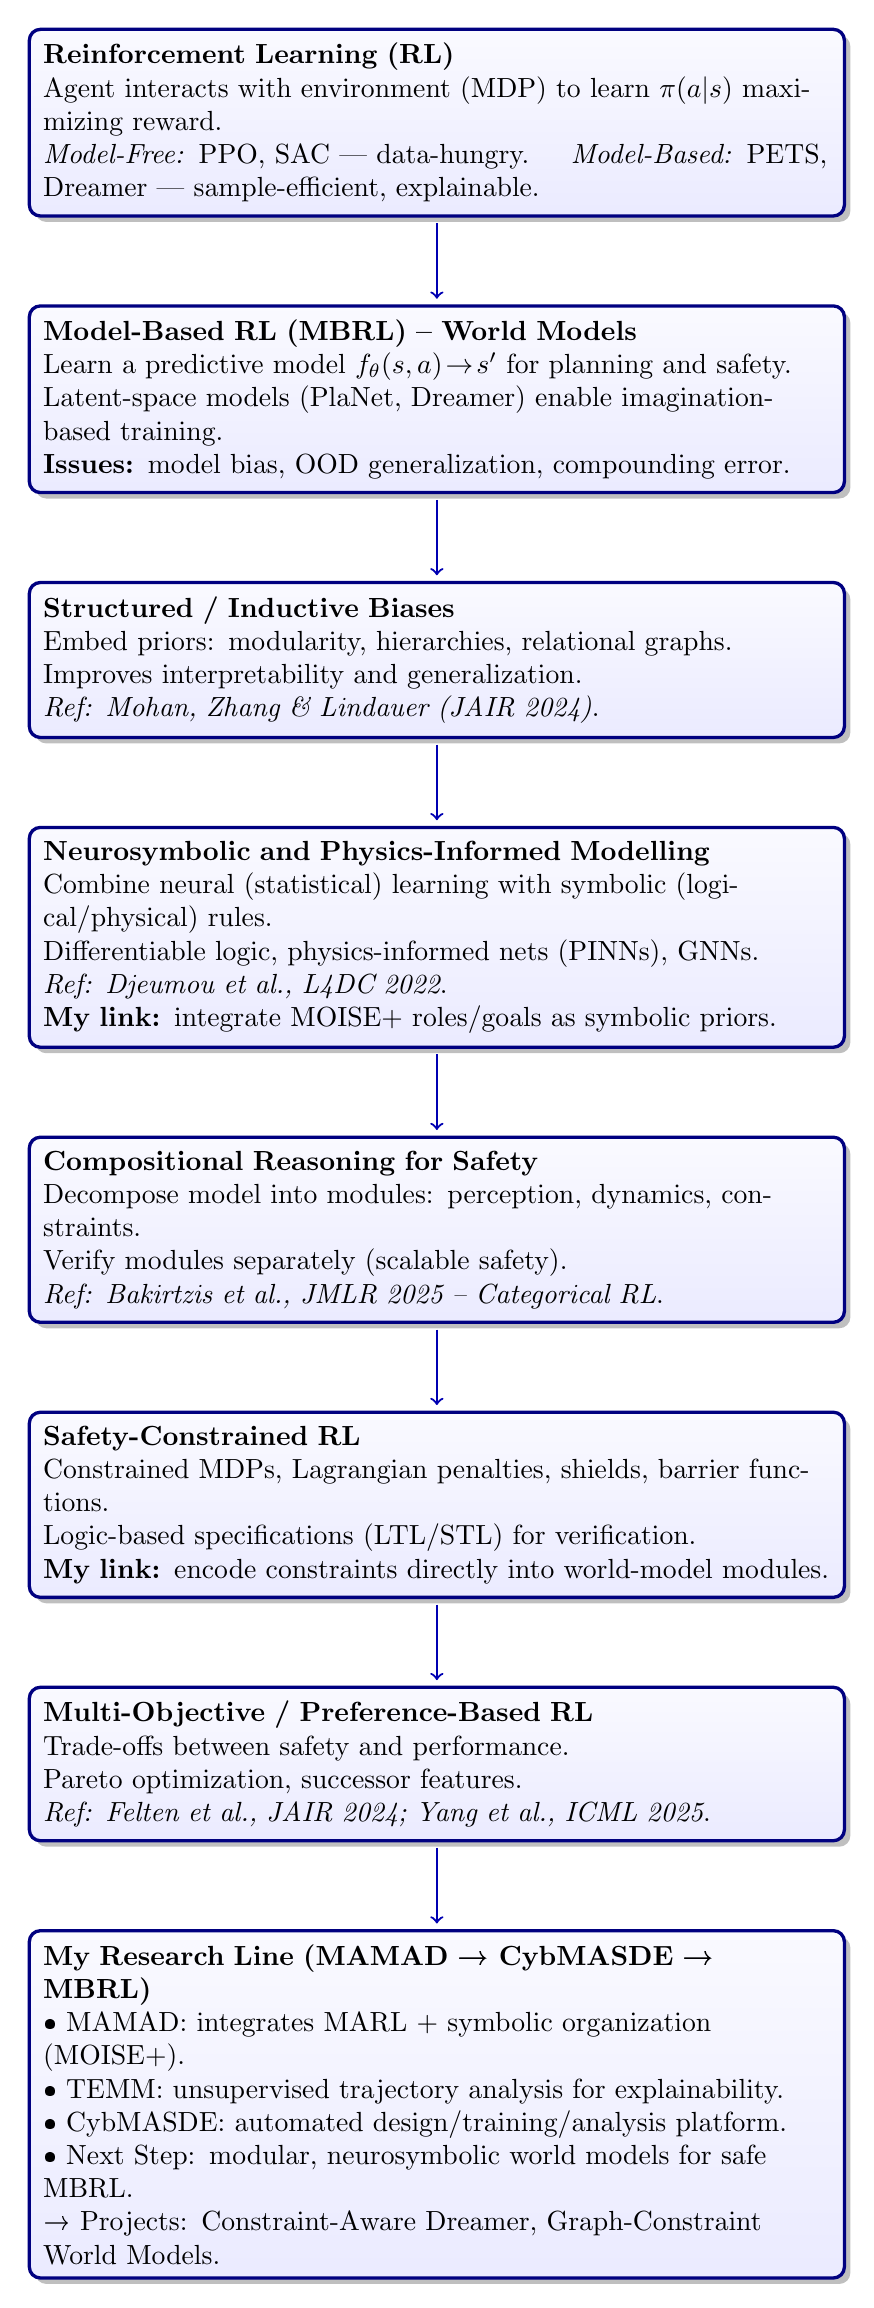
\begin{tikzpicture}[
        node distance=1.1cm and 2.5cm,
        box/.style={
                rectangle, rounded corners,
                draw=blue!50!black, very thick,
                top color=blue!2, bottom color=blue!8,
                text width=10cm, align=left,
                drop shadow, inner sep=5pt
            },
        title/.style={font=\bfseries\large\color{blue!60!black}},
        arrow/.style={->, thick, shorten >=2pt, shorten <=2pt, color=blue!70!black}
    ]

    % Nodes (top to bottom)
    \node[box] (rl) {
        \textbf{Reinforcement Learning (RL)}\\
        Agent interacts with environment (MDP) to learn $\pi(a|s)$ maximizing reward.\\
        \emph{Model-Free:} PPO, SAC — data-hungry. \quad
        \emph{Model-Based:} PETS, Dreamer — sample-efficient, explainable.
    };

    \node[box, below=of rl] (mbrl) {
        \textbf{Model-Based RL (MBRL) – World Models}\\
        Learn a predictive model $f_\theta(s,a)\!\rightarrow\!s'$ for planning and safety.\\
        Latent-space models (PlaNet, Dreamer) enable imagination-based training.\\
        \textbf{Issues:} model bias, OOD generalization, compounding error.
    };

    \node[box, below=of mbrl] (structure) {
        \textbf{Structured / Inductive Biases}\\
        Embed priors: modularity, hierarchies, relational graphs.\\
        Improves interpretability and generalization.\\
        \textit{Ref: Mohan, Zhang \& Lindauer (JAIR 2024)}.
    };

    \node[box, below=of structure] (neurosymb) {
        \textbf{Neurosymbolic and Physics-Informed Modelling}\\
        Combine neural (statistical) learning with symbolic (logical/physical) rules.\\
        Differentiable logic, physics-informed nets (PINNs), GNNs.\\
        \textit{Ref: Djeumou et al., L4DC 2022}.\\
        \textbf{My link:} integrate MOISE+ roles/goals as symbolic priors.
    };

    \node[box, below=of neurosymb] (compositional) {
        \textbf{Compositional Reasoning for Safety}\\
        Decompose model into modules: perception, dynamics, constraints.\\
        Verify modules separately (scalable safety).\\
        \textit{Ref: Bakirtzis et al., JMLR 2025 – Categorical RL}.
    };

    \node[box, below=of compositional] (safety) {
        \textbf{Safety-Constrained RL}\\
        Constrained MDPs, Lagrangian penalties, shields, barrier functions.\\
        Logic-based specifications (LTL/STL) for verification.\\
        \textbf{My link:} encode constraints directly into world-model modules.
    };

    \node[box, below=of safety] (multiobj) {
        \textbf{Multi-Objective / Preference-Based RL}\\
        Trade-offs between safety and performance.\\
        Pareto optimization, successor features.\\
        \textit{Ref: Felten et al., JAIR 2024; Yang et al., ICML 2025}.
    };

    \node[box, below=of multiobj] (mine) {
        \textbf{My Research Line (MAMAD → CybMASDE → MBRL)}\\
        • MAMAD: integrates MARL + symbolic organization (MOISE+).\\
        • TEMM: unsupervised trajectory analysis for explainability.\\
        • CybMASDE: automated design/training/analysis platform.\\
        • Next Step: modular, neurosymbolic world models for safe MBRL.\\
        → Projects: Constraint-Aware Dreamer, Graph-Constraint World Models.
    };

    % Arrows
    \draw[arrow] (rl) -- (mbrl);
    \draw[arrow] (mbrl) -- (structure);
    \draw[arrow] (structure) -- (neurosymb);
    \draw[arrow] (neurosymb) -- (compositional);
    \draw[arrow] (compositional) -- (safety);
    \draw[arrow] (safety) -- (multiobj);
    \draw[arrow] (multiobj) -- (mine);

\end{tikzpicture}
\end{document}
